\chapter{Theoretical Background and Technologies}

\section{LLM-Assisted Planning and Structured Agents}\label{sec:llm-assisted-planning-and-structured-agents}

Large language models are used as reasoning components rather than direct coordinate generators. The planning pipeline decomposes the task into three groups of stages. The first group interprets the room and user brief. The second group converts style intent, required objects, optional objects, and object relations into structured JSON artifacts. The third group prepares solver-ready concepts and selects final gallery variants after geometric validation. This structure makes the LLM output inspectable, replayable, and suitable for ablation, while leaving coordinate decisions to the solver.

\begin{figure}[!htbp]
\centering
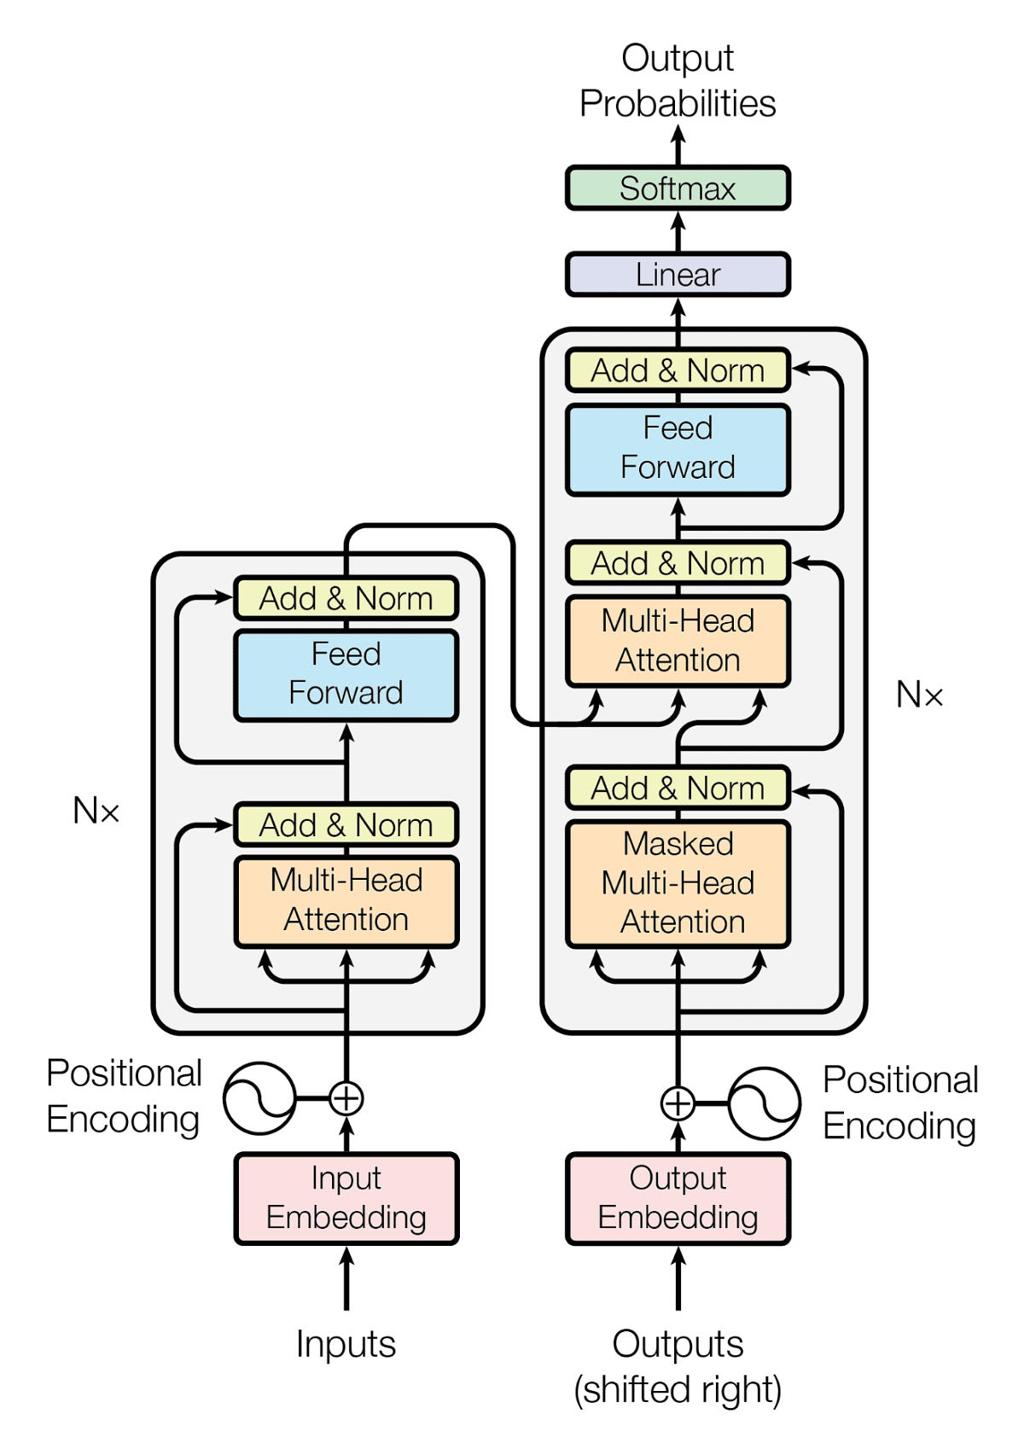
\includegraphics[width=0.78\textwidth]{figures/chapter3/figure_03.png}
\caption{Conceptual Transformer background adapted from Vaswani et al. \cite{al2017AttentionIsAll}. RoomFlow uses provider LLM calls and does not train or modify this architecture.}
\label{fig:3-1}
\end{figure}

\hyperref[fig:3-1]{Figure~3.1} is included as conceptual background for modern LLMs. This thesis does not train or modify a Transformer model. The relevant point is that pretrained language models can convert flexible user briefs into structured design information. In the proposed system, the LLM acts as a semantic planner: it identifies required and optional furniture, infers object relations, interprets style intent, and produces intermediate artifacts such as request contracts and relation plans.

However, the LLM is not used as the only component for final object placement. Its outputs may be plausible in language but still geometrically invalid. Therefore, the system separates semantic planning from geometric placement. The LLM defines what should be placed and why, while the geometric solver checks where objects can be placed by validating room boundaries, collisions, openings, and circulation.

This separation follows recent LLM-based layout systems, where language models are used to plan objects and relations before placement or optimization is applied \cite{al2023LayoutgptCompositionalVisual}, \cite{al2024IDesignPersonalized}, \cite{al2024HolodeckLanguageGuided}, \cite{Littlefair2025FlairgptRepurposingLlms}. In this thesis, the same principle is adapted to an editable application workflow, so the LLM output remains structured, traceable, and usable by the solver, frontend, and evaluation modules.

\section{Indoor Scene Synthesis and Asset-Grounded Layouts}\label{sec:indoor-scene-synthesis-and-asset-grounded-layouts}

Indoor scene synthesis studies how to generate plausible object sets and arrangements for a given room. ATISS models indoor scenes as unordered sets of objects conditioned on room type and floor plan \cite{Paschalidou2021AtissAutoregressiveTransformers}. DiffuScene uses a denoising diffusion model over unordered object attributes, including location, size, orientation, semantics, and geometry features \cite{Tang2024DiffusceneDenoisingDiffusion}. These approaches demonstrate that indoor layout generation is not only a text problem; it also requires structured object attributes and physical plausibility.

The system in this thesis does not train a new scene-synthesis model. Instead, it uses LLM planning and deterministic solving over an inventory of available furniture assets. The inventory connects abstract furniture categories with concrete items, dimensions, style tags, materials, optional prices, colors, and 3D model metadata. If a GLB model exists, the frontend can load it in the 3D preview. If a model is missing or unreliable, proxy geometry is generated so that layout validity does not depend on asset availability.

This asset-grounded approach is suitable for an applied thesis because it keeps the generated design editable. Users can still move objects, compare variants, and reuse the same design structure for preview and image generation. It also avoids the common failure mode in which a generated image looks plausible but no longer corresponds to a concrete object list or editable layout.

The implication for RoomFlow is that the system should not pursue a fully generative 3D scene as the primary output. A fully generative scene can be visually rich, but it may be difficult to edit, audit, or connect to a known furniture inventory. RoomFlow therefore uses a compact, asset-grounded layout as the structural truth and uses generative image models only after the layout has been selected.

\section{Layout-Conditioned Image Generation and Editing}\label{sec:layout-conditioned-image-generation-and-editing}

The image-generation workflow in RoomFlow converts a selected 3D layout preview into a more realistic interior visualization. The provider image model is treated as a black-box text-and-image-conditioned generator \cite{OpenAI2026GptImage2}. Therefore, this thesis does not claim to train or modify the internal image model. The relevant theoretical point is conditional generation: instead of generating an interior image from text alone, the model receives additional visual and structural evidence that describes what should be preserved.

This is important because text prompts are weak at preserving exact spatial layouts. Conditional-control methods show that spatial signals such as edges, depth, or segmentation can improve control over generated images \cite{Ho2020DenoisingDiffusionProbabilistic}, \cite{Rombach2022HighResolutionImage}, and \cite{Zhang2023AddingConditionalControl}. RoomFlow applies this principle at the application level. The selected Three.js view, room shell, openings, visible furniture, object contracts, style-lighting-scenery presets, and preservation constraints are packaged as conditioning evidence. The goal is not exact geometric rendering, but reducing layout drift while improving realism, materials, lighting, and atmosphere.

Image editing follows the same idea of controlled conditioning. Instruction-based editing methods show that an input image and a written instruction can jointly define an edit \cite{Brooks2023Instructpix2pixLearningFollow}. In RoomFlow, each edit request is further constrained by a target object or region, an operation type such as add, remove, replace, or recolor, and preservation rules for the camera view, room shell, openings, and unrelated furniture. The theory point is therefore localized editing with preservation, not retraining a new image model.

\section{Evaluation Metrics for Layout and Image Quality}\label{sec:evaluation-metrics-for-layout-and-image-quality}

The evaluation uses two groups of metrics. Layout metrics check whether a generated layout is geometrically valid, follows the user request, forms a usable room arrangement, and contains enough usable furniture. Image metrics check whether a generated or edited render preserves the selected layout, follows visual presets, performs the requested edit, and avoids unintended changes. Chapter 7 defines the exact scoring protocol, weights, benchmark cases, and ablation-specific stability metrics.

Vision-language models connect visual features with language reasoning by mapping image representations into a language-model reasoning space \cite{Liu2023VisualInstructionTuning}. Figure~\ref{fig:3-2} shows this architecture as background for the evaluation-time VLM checks used in the thesis. In this thesis, this idea is used only for evaluation-time inspection, not as a trained component of RoomFlow. VLM-based inspection judges camera framing, room shell, openings, major objects, and unauthorized additions. The final interpretation combines these checks with preset-fidelity checks and human edit scoring.

\begin{figure}[!htbp]
\centering
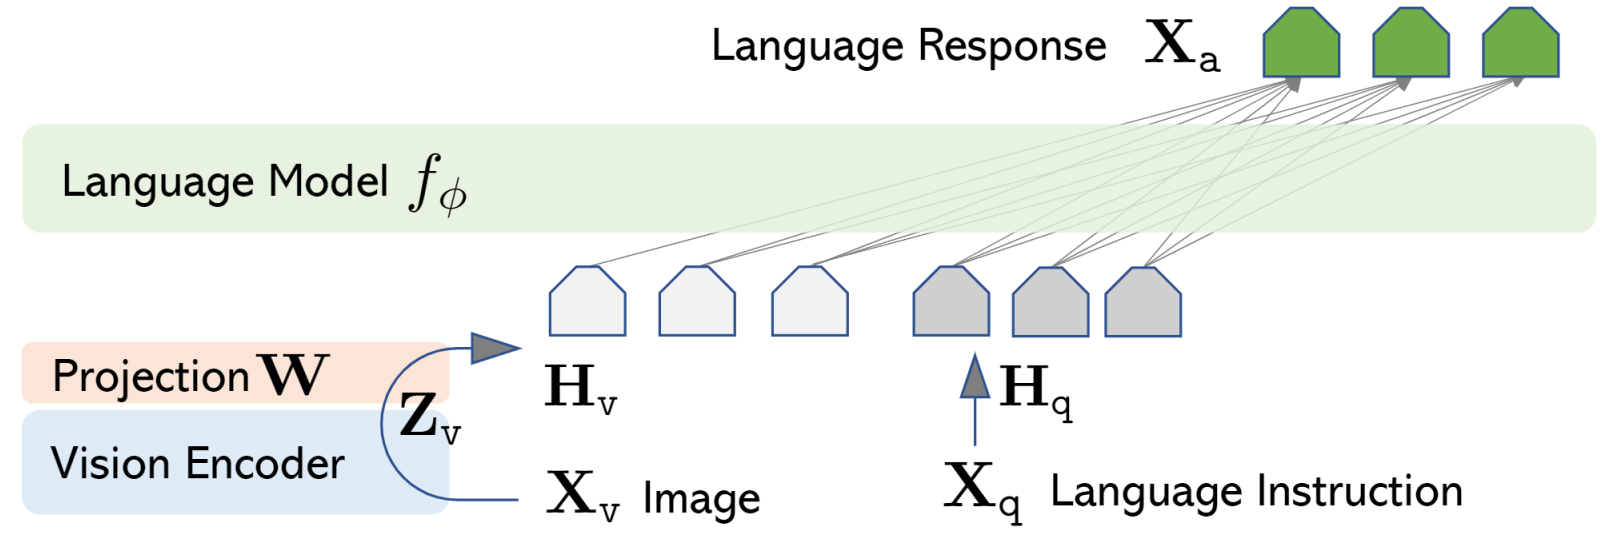
\includegraphics[width=0.94\textwidth]{figures/chapter3/llava_network_architecture.png}
\caption{LLaVA network architecture reproduced from Liu et al. \cite{Liu2023VisualInstructionTuning}. RoomFlow uses a provider VLM only for evaluation-time inspection and does not train or modify this architecture.}
\label{fig:3-2}
\end{figure}

For generated and edited images, traditional full-reference metrics such as SSIM and learned perceptual metrics such as LPIPS are useful references but are not sufficient for this system \cite{Wang2004ImageQualityAssessment}, \cite{Zhang2018UnreasonableEffectivenessDeep}. The actual evaluation therefore combines blank-image checks, provider runtime and token usage, vision-based layout fidelity, and structural preservation. Layout fidelity checks camera framing, room shell, openings, object inventory, object position, object scale, object silhouette, and unauthorized additions. Structural preservation is estimated with edge-map matching, monocular-depth similarity, and DINOv2 patch/object feature similarity, because self-supervised visual features can remain meaningful even when texture and lighting change \cite{al2023Dinov2LearningRobust}. The internal architectures of these perceptual reference models are not reproduced because they are not implemented as system modules; Chapter 7 focuses on the measurable signals they provide for the thesis experiments.

The image-flow metrics also include preset fidelity and edit-specific fidelity. Preset fidelity checks whether the generated image follows the selected style, lighting, and scenery intent. Edit-instruction fidelity checks whether the requested add, remove, replace, or recolor operation was performed, while edit-scope fidelity measures whether changes outside the target region remain limited. These metrics are intentionally strict: a photorealistic image may look good but still fail if it moves the camera, replaces the sofa, changes a window, alters object scale, or edits outside the requested scope.

These metrics also have limitations. Pixel-level and structural metrics may punish a successful render when texture, lighting, or material realism changes the image substantially. Conversely, a conservative edit can obtain high edge or depth similarity simply because it changes too little, even if it fails the requested operation. For this reason, Chapter 7 interprets automated image metrics together with preset checks and human edit scoring rather than treating any single metric as a complete judgment of quality.

\section{Web Technologies Used in the System}\label{sec:web-technologies-used-in-the-system}

The system is implemented as a web application because the target workflow requires interactive editing, long-running AI calls, and persistent artifacts. The frontend uses React, Canvas, and Three.js for 2D editing and 3D preview. The backend uses FastAPI for API endpoints and server-sent events for progress reporting. PostgreSQL stores users, inventory, saved layouts, and generated renders. Chapter 6 describes how these technologies are organized into the final software architecture.
